\section{Приближение функции многочленами}
\subsection{Задача, модель и функция ошибки}
\begin{enumerate}
    \item Допустим, у нас есть функция от одной переменной $f(x)$.
    \item Мы знаем ее значения на каком-то множестве точек (назовём его \textbf{тренировочным множеством}) c некоторым отклонением (шумом) $\varepsilon(x)$
    \item Хотим научиться восстанавливать (хотя бы приблизительно) эту функцию. 
\end{enumerate}

Мы хотим найти набор коэффициентов $(\overline a_0, \overline a_1, \dots, \overline a_n)$, которые  <<приближают>>  исходную функцию.
Пусть 
$$P(x) = \overline a_0 + \overline a_1 x + \overline a_2 x^2 + \dots + \overline a_n x^n \approx f(x)$$

Из-за того, что значения из тренировочного множества неидеально приближают исходную функцию, мы не можем точно определить искомый набор коэффициентов.

Эта проблема подводит нас к новому определению. Введём новую функцию $L(P)$, с помощью которой будем определять, насколько хорошо наша <<модель>> $P(x)$ приближает исходную функцию $f(x)$. 

Назовем $L(P)$ \textbf{функцией ошибки} или \textbf{функцией потерь}. Будем считать, что чем меньше $L(P)$, тем лучше наша <<модель>> приближает $f(x)$. 

Таким образом, минимизируя $L(P)$ будем получать наилучшее приближение функции $f(x)$

Рассмотрим самые часто используемые функции потерь:
    $$L(P) = \frac{1}{n}\sum^n_{i=0} (P(x_i) - f(x_i))^2 \hspace{10pt} \text{--- MSE}$$
    $$L(P) = \sqrt{\frac{1}{n}\sum^n_{i=0} (P(x_i) - f(x_i))^2} \hspace{10pt} \text{--- RMSE}$$
    $$L(P) = \frac{1}{n}\sum^n_{i=0} |P(x_i) - f(x_i)| \hspace{10pt} \text{--- L1 loss}$$
    
\subsection{Переобучение}

Рассмотрим простую функцию $f(x) = 3x^3 - 2x^2 + x + \varepsilon(x)$:

Давайте попробуем приблизить эту функцию многочленом третьей степени: 
\begin{center}
    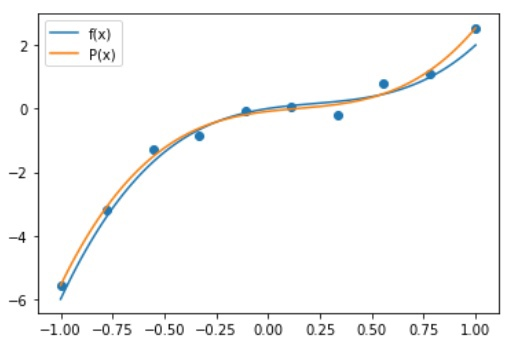
\includegraphics[scale=0.5]{tickets/pictures/polynom3degree.png}
\end{center}
Видно, что мы получили довольно хорошее приближение исходной функции

Попробуем увеличить степень нашей модели до шестнадцати:
\begin{center}
    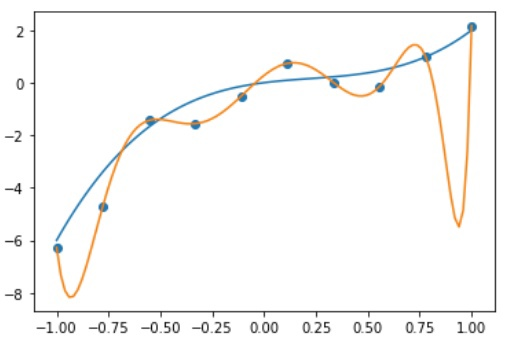
\includegraphics[scale=0.5]{tickets/pictures/polynom16degree.png}
\end{center}

Видно, что модель стала хуже предсказывать исходную зависимость, но при этом на тренировочном множестве выдает идеальные ответы.

Мы столкнулись с проблемой \textbf{переобучения (Overfitting)}.

\subsection{Разбиение на обучающую и тестовую выборку и кросс-валидация}

Как узнать, находит ли исходную зависимость наша модель или переобучается?

Обычно пользуются одним из двух подходов:
\begin{enumerate}
    \item \textbf{Разбиение на обучающую и тестовую выборку (train test split)}
    
    Прежде чем обучать модель, разобьем исходное тренировочное множество на обучающую и валидационную (тестовую) выборки.
    
    Теперь, если мы обучим модель на обучающей выборке, то сможем сравнить значение функции потерь на валидационной выборке, объекты из которой модель не видела при обучении, и на обучающей.
    
    Если эти значения сильно отличаются, то можно говорить о переобучении нашей модели.
    
    \item \textbf{Кросс-валидация}
    Разобьем исходное тренировочное множество на $k$ примерно равных частей.
    Теперь поочередно обучим $k$ моделей на $k - 1$, каждый раз выкидывая новую часть. Если мы посчитаем функцию ошибки для каждой модели на частях, которые не были включены при обучении, а затем усредним, то получим более объективное значение функции ошибки.
    
\end{enumerate}